% arara: pdflatex: { shell: yes }
% arara: bibtex
% arara: pdflatex
% arara: pdflatex: { synctex: on}
% arara: clean: {files: [.aux, .idx, .ilg, .ind, .log, .bbl, .bcf, .ist, .blg, .run.xml]}

% sample.tex
% 
% A sample UMBCposter.
%
% Rouben Rostamian, February 2010

\documentclass[paper=a1paper, dvipsnames, fontmag=0.65]{umbcposter}
\usepackage{color}
\usepackage{enumitem}
\usepackage{colortbl}
\usepackage{tipa}
\usepackage{times}
\usepackage{graphicx}
\usepackage{url}
\usepackage{mdwlist}
\usepackage{amsmath,amsthm,amssymb,bm}
\usepackage{tikz}
\usetikzlibrary{spy,arrows.meta,shapes.geometric,arrows,fit ,plotmarks ,shapes.arrows,decorations.pathmorphing ,matrix,chains,scopes,positioning ,fadings ,patterns ,shapes,snakes,decorations.pathreplacing}
\tikzfading[name=fade out, inner color=transparent!0, outer color=transparent!100]

\usepackage[latin1]{inputenc}
\usepackage{multicol}
 \setlength{\columnsep}{1cm}
\renewcommand{\rmdefault}{pag}

% Turn off indenting
\setlength{\parindent}{0in}

\let\Textsize\tiny
\def\Head#1{\noindent{\Large #1}}
\def\LHead#1{\noindent{\Large  #1}}
\def\Subhead#1{\noindent{\large #1}}
\def\Title#1{\noindent{\VeryHuge #1}}

\newcommand{\Line}{\hrulefill\par}
\newcommand{\Space}{\vspace{0.1cm}}

\newcommand{\myvec}[1]{\pmb{#1}}
\newcommand{\mleEst}{\hat{\Theta}_{\textrm{MLE}}}
\newcommand{\est}{\hat{\Theta}}
\newcommand{\fn}[2]{#1 \left( #2 \right)}
\newcommand{\samplespace}{\mathbb{S}}
\newcommand{\argmax}{\arg\max}
\newcommand{\definedas}{:=}


\begin{document}

\newcommand{\mytitle}{
\begin{tabular}{l}
\begin{minipage}[t]{0.5\linewidth}
		\huge Comparing John Walker's 18th century\linebreak grammatical categories against those of\linebreak today with Treetagger 
\end{minipage}
\hspace{0.1cm}
\begin{minipage}[t]{0.4\linewidth}
	\large Francois {\bf HUANG}\\
	\large Blanche {\bf MIRET}\\
	\large Preethi {\bf SRINIVASAN}\\
	\large Dao {\bf THAUVIN}\\
	\large Universit\'e de Paris\\ 
\end{minipage}\\
\begin{minipage}[t]{0.8\linewidth}
 Ce travail est l'\oe{}uvre conjointe d'\'etudiants de la Licence Informatique et de la Licence d'\'Etudes Anglophones de Paris Diderot.\\ Il a \'et\'e financi\`erement support\'e par le programme  IdEx Universit\'e de Paris ANR-18-IDEX-0001
 \end{minipage}
\end{tabular}
}

\posterinit{
	%grid,
	columns = {2},
	title align = {left},
	background style = {left color = white!90!gray, right color = white},
	title = \mytitle,
	right logo = {
\includegraphics[height=0.9\headheight]{Logo_Universite.png}},
	box/border style = {draw = black},
    box/header font = {\Large\bf},
	box/header font color = {black},
	box/header style = {top color = white!50!gray,
	bottom color = white!50!gray, line width=1pt},
	box/body style = {bottom color = white!80!gray, top color = white!90!gray},
	box/all rounded,
}

\boxit{col = 0,  span=2,at top, name = introduction}{Introduction}{
  As it is very well known, Treetagger (\textit{Helmut Schmid}, 1996) is a tool that is widely used in the Natural Language Processing domain to annotate multilingual corpora with POS taggers and lemma information. The purpose of this study is to find out whether Treetagger could learn the grammatical categories of John Walker's \textit{Critical Pronouncing Dictionary }(1791).
}
\boxit{col = 0, below of=introduction, name = corpus}{Data}{
  \begin{center}
\textbf{TreeTagger with Walker's grammatical categories}\\[3mm]

	- \underline{Lexicon :} Words defined by J. Walker in his dictionary\\[2mm]
	- \underline{Tagset :} Walker's grammatical categories\\[2mm]

\textbf{TreeTagger with Brown Corpus' grammatical categories}\\[3mm]

	- \underline{Lexicon :} Words extracted from Brown Corpus\\[2mm]
	- \underline{Tagset : } Grammatical categories from Brown Corpus\\[3mm]

\noindent\rule{4cm}{0.4pt} \\[2mm]

\underline{Training Data }: Extract from Brown Corpus\\[2mm]
\underline{Test Data} : Two extracts: one from Brown Corpus, different from the training data and tagged, and another from some definition written by Walker in his Dictionary.
\end{center}

}
\boxit{col = 0,span=1, below of = corpus, name = workflow}{Methods}{
  \begin{center}
- Create a \textbf{mapping table} from Brown Corpus tagset to Walker's tagset and \textbf{apply it on our training data}.  \\


\begin{center}
\begin{tabular}{c|c}
\hline
 \rowcolor[gray]{.75}
\textbf{Treetagger's POS tags} &  \textbf{Brown Corpus's POS tags} \\
\hline
art  &  at, dt \\
\hline
adj  &  jj, dti, ap, dts, jjt, jjr, jjs \\
\hline
pret  &  vbd, dod, bed, bedz, hvd \\
\hline
s  &  nn, nr, nns, nps \\
\hline
conj  &  in, cs, cc, dtx \\
\hline
prep  &  in, to \\
\hline
part.pass.  &  hvd, vbn, md \\
\hline
tp (third person)  &  vbz, bez, hvz, doz \\
\hline
v.  &  bem, vb, hv, be, do, ber \\
\hline
adv.  &   rb, ql, abx, abn, abl, ex \\
\hline
pron.  &  pps, ppo, pn, wps, ppl, wdt \\
\hline
part.  &  vbg \\
\hline
interj.  &  uh \\
\hline
\end{tabular}
\end{center}

- \textbf{Train TreeTagger} with our training data with Walker's tagset  \\[2mm]

- \textbf{Train TreeTagger} with our training data with Brown Corpus tagset \\[2mm]

- \textbf{Run }both trained Taggers on our test Data \\[2mm]

- \textbf{Compare} the Brown Corpus' test data \textbf{results} to the \textbf{original tagged corpus} \\[2mm]

- \textbf{Check} the tags obtained by the other \textbf{result }

\end{center}

}
\boxit{col = 0,span=1, below of = workflow, name = remarks}{Remarks on Walker's Dictionary}{
  \begin{center}

- Brown Corpus's tagset and grammatical categories of Walker's dictionary \textbf{don't match}
because many categories \textbf{changed} or simply \textbf{disappeared} over the course of time. \\[2mm]

- 37895 words were tagged and 879 were not in Walker's Dicitonary\\[2mm]

- The tag \textbf{contraction}  hasn't been used for every words which required it. \\
Examples :  \textit{NE'ER} is a poetical contraction for Never. Walker declared it as an adverb.\\
\textit{TA'EN} is a poetical contraction for Taken. Walker declared it as a contraction.

\end{center}





}
\boxit{col = 1,span=1, below of = introduction, name = preparingTT}{Preparing TreeTagger}{
  \begin{center}
\textbf{ About our lexicon from Walker's dictionary:}\\[1mm]
	
- We \textbf{added} some proper nouns, punctuation marks and cardinal numbers from our training set.\\
- We \textbf{fused} some categories to match brown corpus categories\\
- Some categories have \textbf{disappeared}, such as solemn nominative plural. ( Hapax: Ye ), and A negative or privative termination. ( Hapax: Less ).\\
- 33688 words\\[2mm]

\textbf{About our lexicon from Brown Corpus:}\\[1mm]

- 56057 words\\[2mm]

\textbf{About our training set :}\\[1mm]
- about 1500 sentences\\
- 28639 words (including punctuation marks)

\end{center}

}
\boxit{col = 1,span=1, below of = preparingTT, name = results}{Results}{
  \begin{center}
\large
\textbf{Differences between Brown corpus tagging and our tagging :}\\[4mm]
\normalsize

\underline{With Walker's tagset :}\\[2mm]
	- 1590 failures on 2332 tags.\\
	- A big amount of s. with 1300 failures in our tagging.\\
	- Only 8 tags have been used : adj., s., SENT, pron.pers., CD, NP, art., interj.\\[4mm]
\underline{With Brown Corpus's tagset :}\\[2mm]
	- 91 failures on 2332 tags.\\[4mm]

\large
\textbf{Manual tag check for the other result :}\\[2mm]
\normalsize

\underline{With Walker's tagset :}\\[2mm]
	- 35 failures on 54 tags.\\
	- 25 failures with s. in our tagging.\\[4mm]
\underline{With Brown Corpus's tagset :}\\[2mm]
	- 5 failures on 54 tags.\\
	- 2 failures about ;\\[2mm]
	
		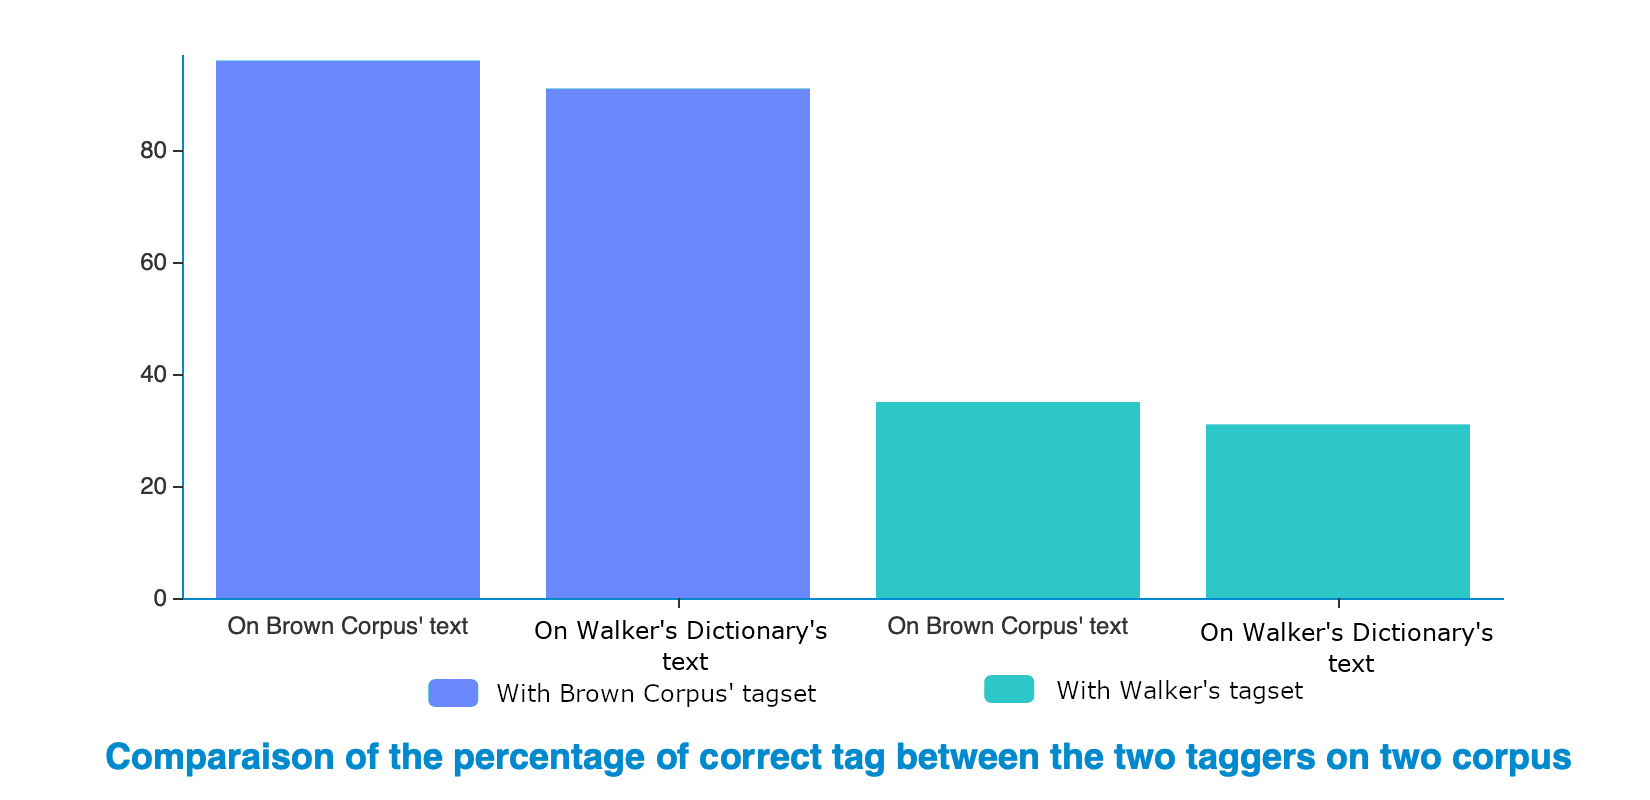
\includegraphics[width=9cm]{chart3.png}

\end{center}

}
\boxit{col = 0,span=2, below of = remarks, name = discuss}{Discussion about the results}{
  \begin{center}
For our Tagger with Walker's dictionary tagset :\\[2mm]
- Size of the tagset : \textbf{19 tags}. As reference, the Brown Corpus tagset has \textbf{86 tags}. Therefore, our \textbf{small number of tags} probably impacts the result.\\

- \textbf{Lost} of many useful tags from Walker's Dictionary. 
We could fix that by \textbf{tagging manually} the training set to keep most of the tags.\\

- Training on a \textbf{bigger training} set could give a better result. Most of the tags not used are rare tags that don't often appear in the training set. For example, the tag sp (for second person) appears only five times.\\[2mm]

Finally, without taking account of those remarks, it seems that \textbf{Walker's dictionary tagset can't be applied to TreeTagger} with the same accuracy as it has with modern parameter files.
\end{center}


}
\small

\boxit{col = 0,span=2, below of = discuss, name = references}{References}{
  \begin{multicols}{2}

\begin{center}
1. J. Walker. \textit{A Critical Pronouncing Dictionary}, 1824. \\[2mm]

2. N. Trapateau. \textit{A Critical Pronouncing Dictionary} from J. Walker xml file\\[2mm]

3. W. N. Francis and H. Kucera. \textit{Brown Corpus}\\[2mm]

4. The project's Github : https://github.com/daothauvin/TreeTaggerWithWalker
\end{center}
\end{multicols}
}



\end{document}

